\documentclass[12pt]{article}
\usepackage{amsmath}
\usepackage{amssymb}
\usepackage{setspace}
\usepackage{graphicx}
\usepackage[margin=1in]{geometry}
\newcommand{\del}{\nabla}
\doublespacing
\begin{document}

\title{Nonlinear Analysis of Nonverbal Behavior Synchronization}
\author{Howon Lee}
\maketitle

\section{Abstract}
There exists a literature dealing with time series analysis in the nonlinear sciences in the case of synchronization, or the adjustment of rhythms of oscillating objects to coincide with each other due to weak interaction. We attempt some of these methods in analyzing an instance of the phenomenon of interpersonal synchrony in human movement data. We also propose a mapping from time series to networks with a deterministic inverse, useful for exploratory analysis.

\section{Introduction}

Before defining what we mean by synchronization in this context, we note that there exists a long history of the study of synchronization outside of social science. Synchronization was first reported in physical systems by Huygens in 1665. He saw that two pendulum clocks in the boat that he was testing the clocks in were mysteriously ticking in unison, and found that the cause was a support beam which connected the clocks, which moved imperceptibly and therefore maintained the synchronization\cite{physsync}.

Centuries later, the physical and biological systems which were later found to synchronize include mechanical rotators, lasers, fireflies emitting synchronous patterns of light, synchronous contraction of heart cells, synchronization of human circadian rhythm to a solar light cycle, and synchronous interaction of human beings\cite{syncreview}, \cite{physsync}.

Now, we should define the terms. Interpersonal synchrony is defined in the social science literature as individuals' temporal coordination during social interaction\cite{socialsync}. In the physical sciences, synchronization is defined as an adjustment of rhythms of oscillating objects due to weak interaction, with generalizations possible for chaotic systems, which depend upon a phase of the chaotic system existing\cite{physsync}.

Although social synchrony is one of many other synchronies, many of which do not necessarily serve a function of any kind, it is observed that social synchrony serves a function in human social groups. There exists evidence that synchronization acts as a cooperation-inducing mechanism\cite{coop}, that it acts to induce rapport\cite{rapport}, and that it in actuality, independent of its effect on rapport, enhances the ability to pursue joint goals in tandem for those who are synchronized\cite{goals}. This suggests immediately that it must be measured in a systematic way, to study phenomena of that kind.

In the beginning of the social synchronization literature, most psychologists did not use the then-developing automated signals processing techniques for the detection and measurement of synchronization, instead using manual methods to detect and rate the presence or absence of synchronization, with trained raters and validated measuring systems\cite{manual}. Although these measurements have been validated\cite{manualval}, they depend upon human raters and therefore are less replicable and less convenient than automated systems.

Given that the signals created by an individual during social interaction have a phase, and social interaction can be construed as a weak interaction between the two individual systems, it should be clear that the definition of interpersonal synchrony given in the social psychological literature is a subset of the definition given in the physics literature. This has often been noted\cite{socialsync}, and has therefore spawned a cross-disciplinary field wherein signals processing techniques are used to measure interpersonal synchrony.

As a specific instance of a domain where signals processing techniques are used, a large problem in synchronization is the definition of the signal itself and its extraction from observations of social interaction. To this end, many methods have been used, including extraction of coordination of movement features and speech features\cite{movementfeatures}, movement of single and dyadic body parts\cite{movementparts}, image processing techniques\cite{imageprocessing} and video tracking techniques\cite{videotracking}.

An important analogy exists between the collection of time series data about the physiology of the body in order to assess synchrony and the collection of time series data about the body in order to assess health. Indeed, there exists a literature on the synchronization properties and the time series analysis of heart rate variability which we have derived much inspiration from, not necessarily in the usage of correlational metrics, for which there is a literature dealing in social synchronization, but more sophisticated metrics for which there is not such a literature\cite{hrv1}. The essential premise is that we treat social synchronization as an instance of an abstract problem of physical synchronization, which justifies using measures used by other physiological measurements.

It is also important to note that there exists a literature which uses various nonlinear methods to track nonverbal synchronization. Recurrence analysis, which is also from nonlinear dynamical systems, provides a graphical representation of the coupling of systems represented by time series, and is used by \cite{webber}, \cite{musicians} and \cite{puzzles} for detecting postural synchronization. \cite{richardson} modelled the interpersonal coordination of two people rocking together on rocking chairs side-by-side as a coupled dynamical system.

This project will attempt to use some of the already existing tools for the analysis of time series data on nonverbal tracking time series data, as well as apply some tools which have not previously been used to analyze synchronization in such time series data of social synchronization in a nonverbal task.

We can take the problem at hand as trying to find hidden structure in the unlabeled time series we are given, where the hidden structure is any present synchrony. Therefore, this can also be construed as an unsupervised learning problem.\cite{socialsync}.

One might wonder why the existing methods of measurement of synchronization do not already serve for the purpose of measuring synchronization of body movements. They do not serve for the same reasons that they do not serve in physical time series. That is, they are fundamentally \emph{linear} measures of the relation that they have to each other, meaning that measuring only correlation implicitly puts in the assumption that an affine transform relates the two signals to each other. It is possible to learn about higher order dependences if correlations of higher moments are used, but this becomes rapidly time-consuming very quickly\cite{pompe}.

\begin{figure}\label{fig:nonlinearity}
  \begin{center}
    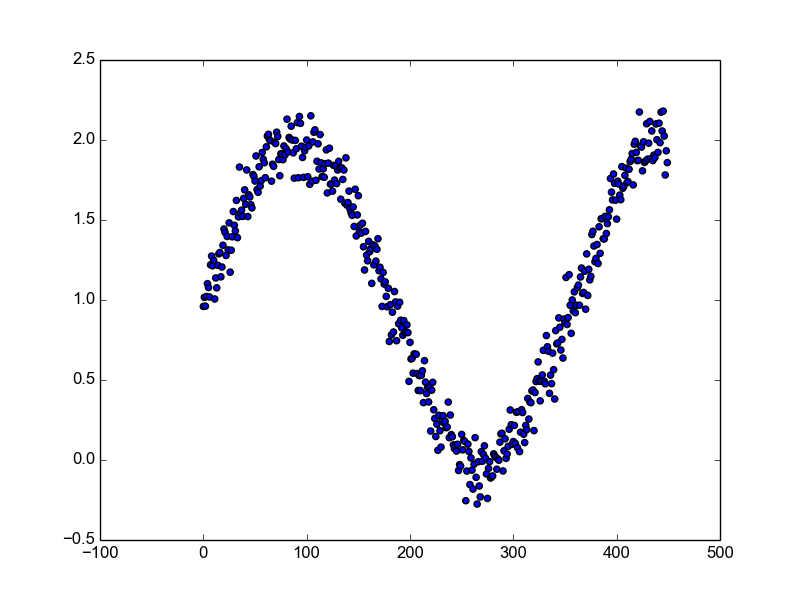
\includegraphics[scale=0.5]{mi_ex}
  \end{center}
  \caption{Example of simple nonlinear relation between two variables}
\end{figure}

One example from \cite{anscombe} which should help develop a theoretical intuition about nonlinearity and synchronization is the sine wave relation example. Consider the figure \ref{fig:nonlinearity}. According to a linear correlation measure, taking the whole domain of $x$ into account at once, the two variables $x$ and $y$ cannot disprove the null hypothesis of independence ($p=0.45$), but by inspection, one can say that actually $y = sin(x) + \epsilon$, where $\epsilon$ is a small amount of Gaussian noise. But nonlinear measures \emph{will} take this nonlinear relation into account. For example, mutual information will say that the mutual information between the two variables $x$ and $y$ is 7.5 bits, which indicates that the variables determine each other to a great degree.

In the psychological literature dealing with referential behavior, or behavior which adapts to some process or set of events or plan \cite{pressing}, there exist two theoretical schools towards the modelling of the feedback systems which are presumed to allow synchronization with respect to a referent: information processing theories and dynamical systems theories. Information processing theories tend to deal with participant responses as discrete time series, and fit to data which is compatible with this paradigm (tapping studies, for example). Dynamical systems theories tend to deal with participant responses as trajectories in a phase space and deal with continuous movements as data \cite{syncreview}.

There exist unifications \cite{pressing} which use the formalism of control theory to include both sorts of models as special cases. In that same paper, some evidence of nonlinearity (specifically, difficulty finding a low correlation dimension and a small but positive Lyapunov exponent, with the caveat that the cardinality of the data was small) which could not be fitted with a linear autoregressive moving average approach was found. \cite{schulze} notes that there are overfitting difficulties with manually incorporating a nonlinear perception detection threshold into a second-order autoregressive moving average model which is to be fit to data.

However, in the \emph{measurement} of degrees of synchronization, or of the experimental discernment of synchronization state, it does not necessarily follow that avoiding the assumption of linearity is as intractable as fitting a nonlinear \emph{model} would be.

Lagged correlation is the most common measure of synchrony in social science. We will examine those in this project as a first pass. Then, we will go into recurrence methods, spectral coherence, Hilbert transforms and transformation into networks.

\subsection{Data Description}

Participants were drawn from the student population at a medium sized West Coast university in the United States and completed the experiment for course credit or \$15 in cash. 110 participants signed informed consent and were paired with another participant to complete a cooperative task.  Of the resulting 56 pairs, eight pairs were discarded due to recording failure, and one partner refused consent, leaving 47 pairs. 13 of these pairs were female/female, 25 of them were female/male, and 9 of them were male/male.

The data was collected as the angle descriptions of a Microsoft Kinect, which outputs many time series for the angle and positions of the heads and body parts (torso, arms and legs) of users, and was preprocessed according to \cite{andrea}.

A problem with the data is that it was missing in places. Because of the differencing in preprocessing which we did, an interpolation would not have been prudent, because an interpolation would have claimed that the original time series had been steadily increasing, which is not necessarily warranted. Therefore the missing data was construed as 0's, because this would be a simple interpolation in the original time series, before preprocessing.

\section{Time Domain Analysis}

\subsection{Correlation Analysis}

When we say \emph{correlation}, in most cases, we mean \emph{Pearson's correlation}, or the \emph{Pearson product-moment correlation coefficient}.

Three fundamentally correlational analyses were tried: time-lagged cross-correlation, Poincare plots and an ad hoc method based on taking the slopes of the change of shape of the data-containing ovals of Poincare plots.

One analysis commonly used with relaxation oscillators (like ECG data) is the Poincare map, not to be confused with the Poincare plot. However, because there are not clear demarcations as to where each oscillation is, the Poincare map is less suited to this dataset and will not be used\cite{physsync}.

\subsubsection{Time-Lagged Cross-Correlation}

This part is a re-analysis of the work from \cite{andrea}, but as stated before, only using the head angle. As in \cite{andrea}, Pearson's correlation was taken on a window of 400 frame data points(50 seconds) and then shifted for consecutive lag times according to \cite{framedifferencing}.

\begin{figure}\label{fig:lag_correlation}
  \begin{center}
    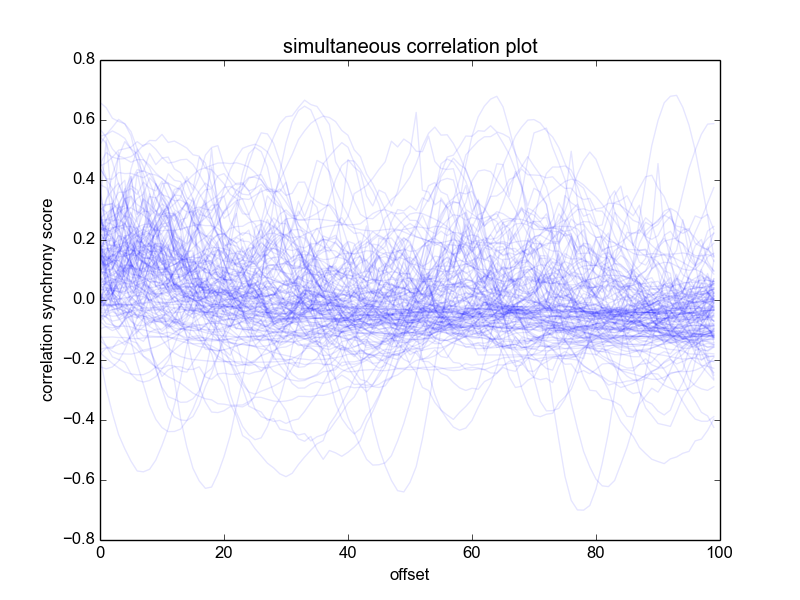
\includegraphics[scale=0.6]{correlation_mc}
    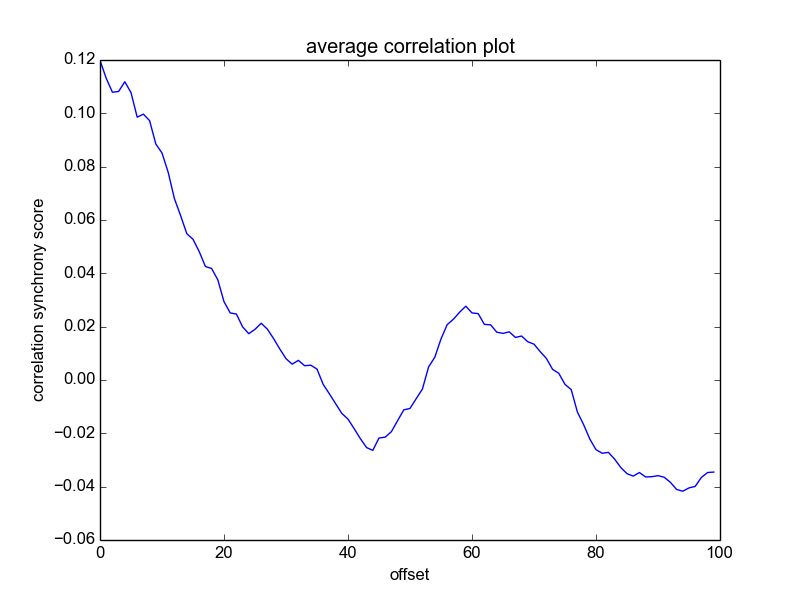
\includegraphics[scale=0.6]{correlation_summary}
  \end{center}
  \caption{Lagged correlation of all data and pointwise averages of lagged correlation}
\end{figure}

\subsubsection{Poincare Plots}

A Poincare plot\cite{hrv1}, not to be confused with the Poincare map, plots the variables in a time series in a certain order to see if there is self-similar structure in that time series. For a time series which exists as a series of variables indexed by time:

$$x_t, x_{t+1}, .... $$

It plots on the first axis the first members of a sliding window bigram composed of the paired members of the time series and on the second axis, the second members of that bigram.

Alternatively and equivalently, a Poincare plot can be thought of as a 2-dimensional reconstructed time series phase space which projects the reconstructed attractor\cite{kamen}.

In the heart rate variability literature, a summary statistic of Poincare plots is often used. Although the time series in the heart rate variability measure is the oscilloscope measure of the heart beat at a certain point in its waveform, we use it also as a summary measure of the Poincare plot. Although the Poincare plot itself is a nonlinear technique, the summary measure is a linear measure\cite{kamen}, defined by fitting an ellipse to the RR interval. The center of the ellipse is held to be at the mean value of the cloud, and the standard deviations of the point cloud with regards to the $x_t = x_{t+1}$ line and the line perpendicular to that line at the center of the point cloud are calculated: those two values, SD1 and SD2, are the measures. These can be related directly to autocovariance\cite{kamen}.

Inspection of the plot itself has more value than simply observing the summary measure, however. The dispersion of points perpendicular to the line $x_t = x_{t+1}$ represents the short-term variability and the dispersion parallel to the line represents a longer-term variability. But this is not the only thing that the Poincare plot can show: intermittent features will show up as small islands of points athwart the main cloud, for example, which the measure doesn't handle well.

\begin{figure}\label{fig:ellipse_histogram}
  \begin{center}
    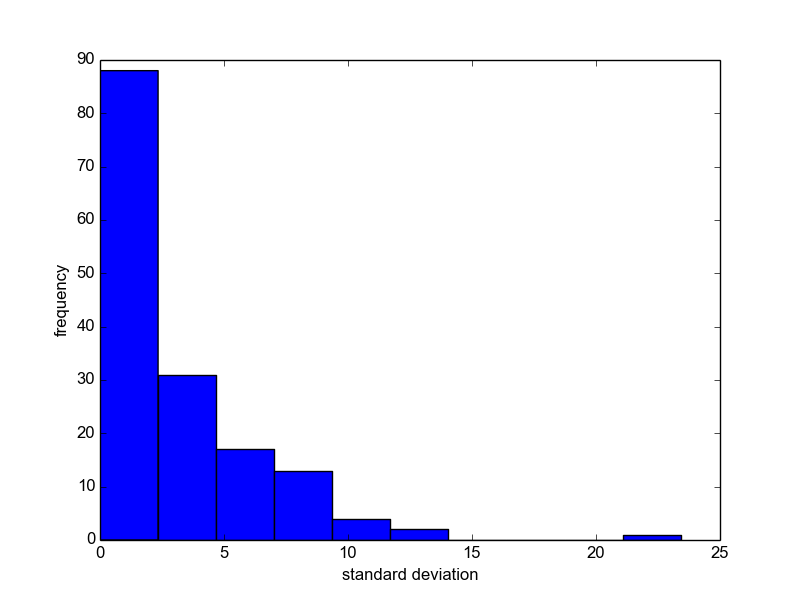
\includegraphics[scale=0.6]{sd1_histogram}
    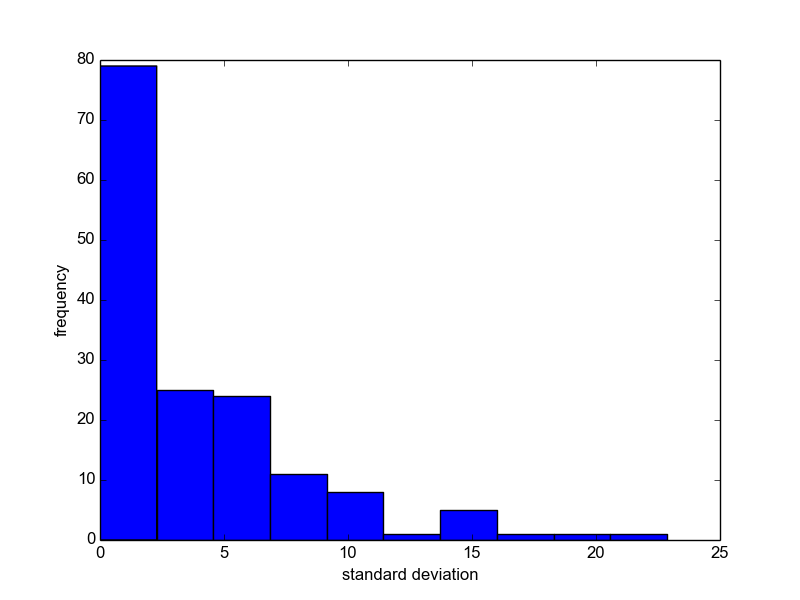
\includegraphics[scale=0.6]{sd2_histogram}
  \end{center}
  \caption{Histogram of SD1 and SD2 in dataset}
\end{figure}

\begin{figure}\label{fig:poincare_plots}
  \begin{center}
    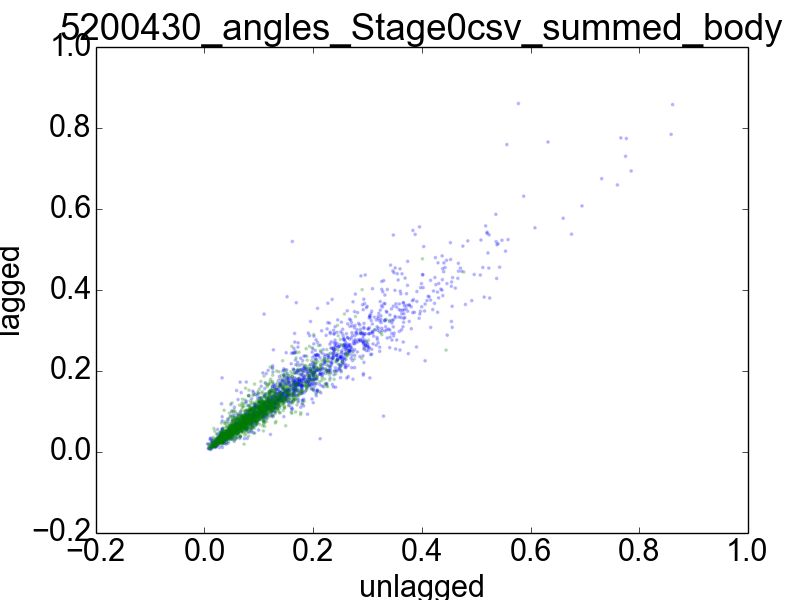
\includegraphics[scale=0.4]{poincare_1}
    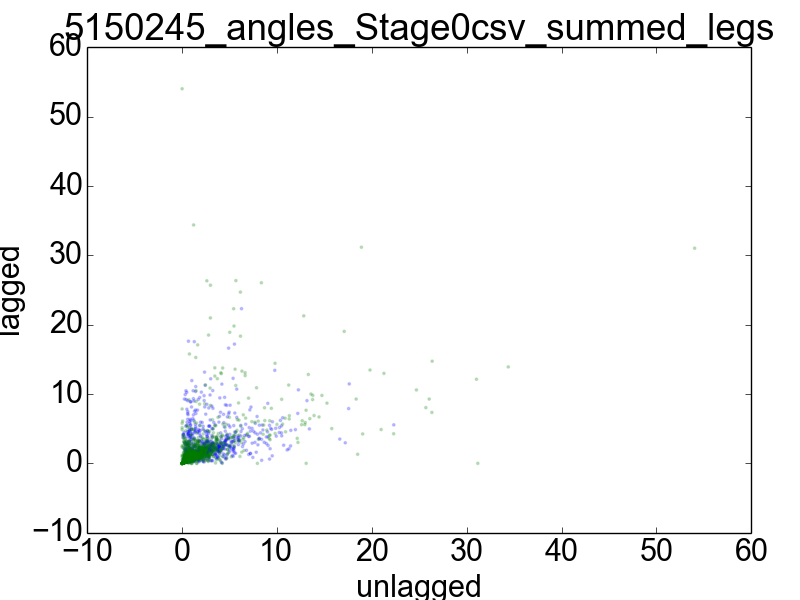
\includegraphics[scale=0.4]{poincare_2}
    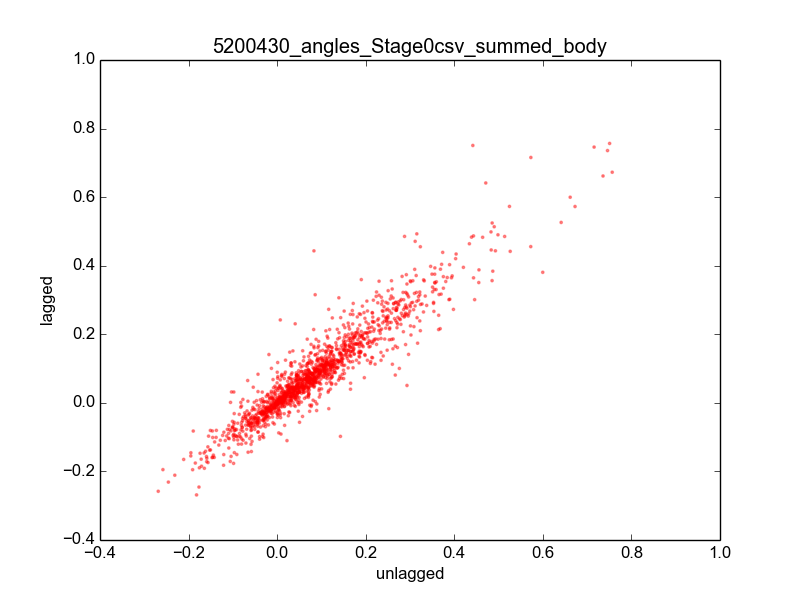
\includegraphics[scale=0.4]{poincare_3}
    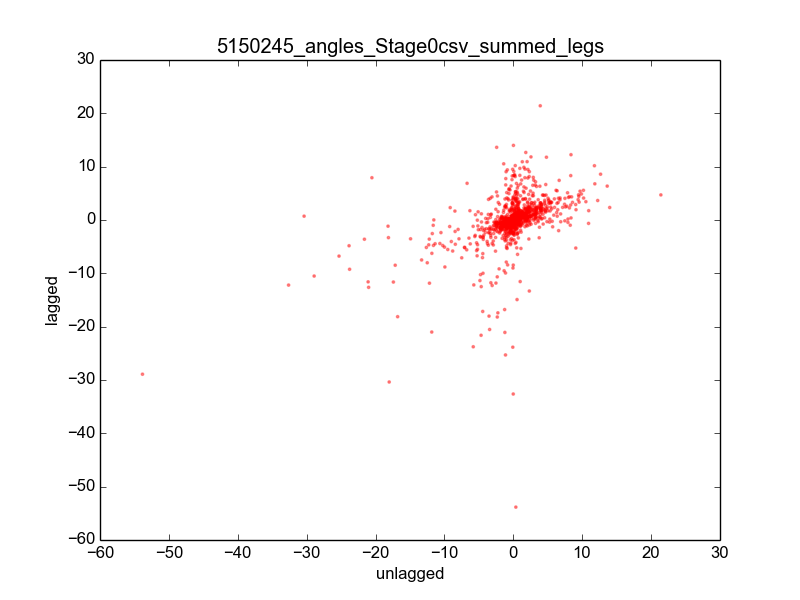
\includegraphics[scale=0.4]{poincare_4}
  \end{center}
  \caption{Example Poincare plots from real data. The first two plots plot both series in a pair, the last two plots plot the difference between both series. Nonlinear structure can be seen in the very last plot.}
\end{figure}

\subsection{Mutual Information Analysis}

Mutual information is important as a measure because it measures the lack of independence of two random variables, as opposed to correlation, which merely measures whether two random variables covary linearly, and therefore is not sensitive to more complex relations as mutual information is.

In order to introduce mutual information, we must introduce Shannon information and Shannon entropy\cite{nnmi}.

Shannon information is defined on a measurement drawn from some set (let the set be discrete, $X \in {1 ... n}$, for ease of notation: there exist continuous analogues). Given that measurement from some set, the Shannon information in bits is defined as:

$$ -\log_2 P_X(i) $$

where $P_X(i)$ is the probability that a measurement will find the system in state $i$. That is, a lower probability answer is more surprising, and therefore more information is found in it.

Shannon entropy, denoted $H(X)$ is defined on a data stream (a measurement stream) $X$. It is the average amount of information contained in every message received, and so is also measured in bits. An easy intuition about entropy can be gained by noting that a \emph{fair} coin flipping process is the most entropic possible coin flip, because we are most surprised by it. Formally, entropy is:

$$H(X) = -\sum_i P_X(i) \log_2 P_X(i)$$

Information and entropy are also defined on joint probability distributions in an analogous way. The information of a joint probability distribution on variables $X$ and $Y$ is:

$$ -\log_2 P_{XY}(i, j) $$

And the entropy, therefore, is:

$$H(X, Y) = -\sum_i \sum_j P_{XY}(i, j) log_2 P_{XY}(i, j)$$

Now, if we sample two random variables simultaneously, the relationship has a quantity defined upon it which is called the \emph{mutual information}. Because it is defined on the relation, it has an auto-mutual information variant and a cross-mutual information variant, like correlation does. However, mutual information measures something different, which is the \emph{information which one of the random variables gives about the other random variable}. It is defined as:

$$I(X, Y) = H(X) + H(Y) - H(X, Y)$$

And one sees that this quantity is symmetric with respect to $X$ and $Y$. Note that two linearly related variables will have a high mutual information \emph{in addition} to a high correlation coefficient.

Because we are dealing with real data, mutual information must be estimated from probability distributions represented as histograms. This is problematic in high-dimensional data, owing to the curse of dimensionality\cite{bellman}. Also, it is the case that the measure itself depends upon an intelligent discretization, which does not make the individual buckets of the histogram too sparse with data\cite{alzheimersmi}. We discretized with 64 buckets, which was recommended for a time series similar in size and range as ours by \cite{alzheimersmi}.

\subsubsection{AMI and CMI}

Auto mutual information (AMI) and cross mutual information(CMI) are the mutual information analogs to autocorrelation and cross correlation. They have the same advantages over the correlation variants as mere mutual information itself has to correlation. Like lagged correlation, mutual information is symmetric with respect to the compared time series.

\begin{figure}\label{fig:lag_cmi}
  \begin{center}
    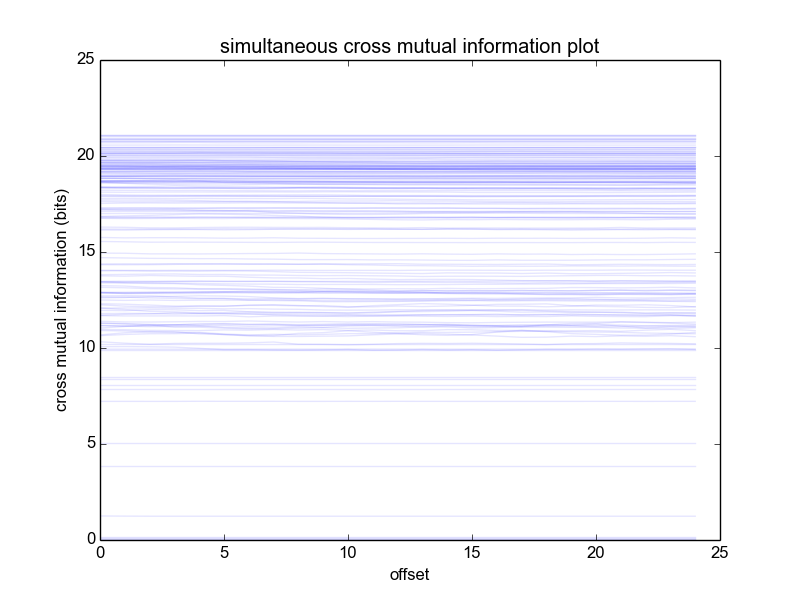
\includegraphics[scale=0.4]{cmi_mc}
    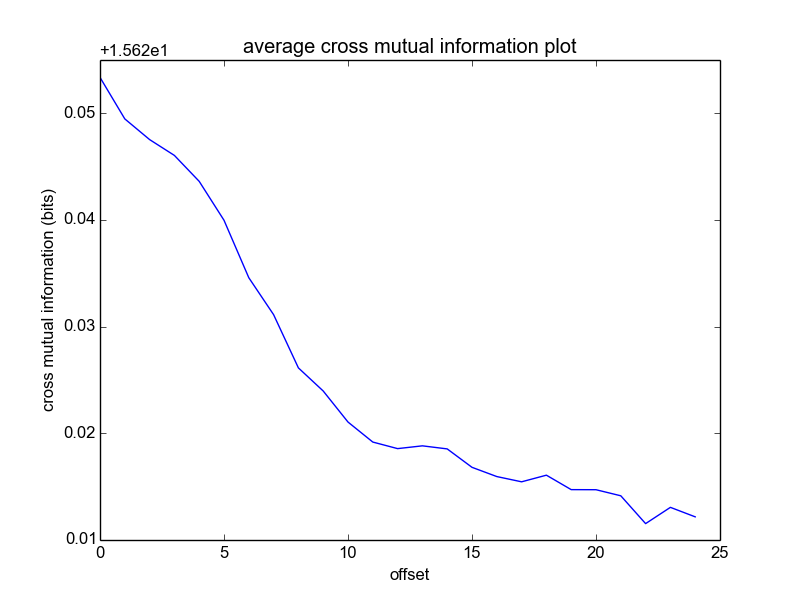
\includegraphics[scale=0.4]{cmi_summary}
  \end{center}
  \caption{Lagged cmi}
\end{figure}

\begin{figure}\label{fig:lag_ami}
  \begin{center}
    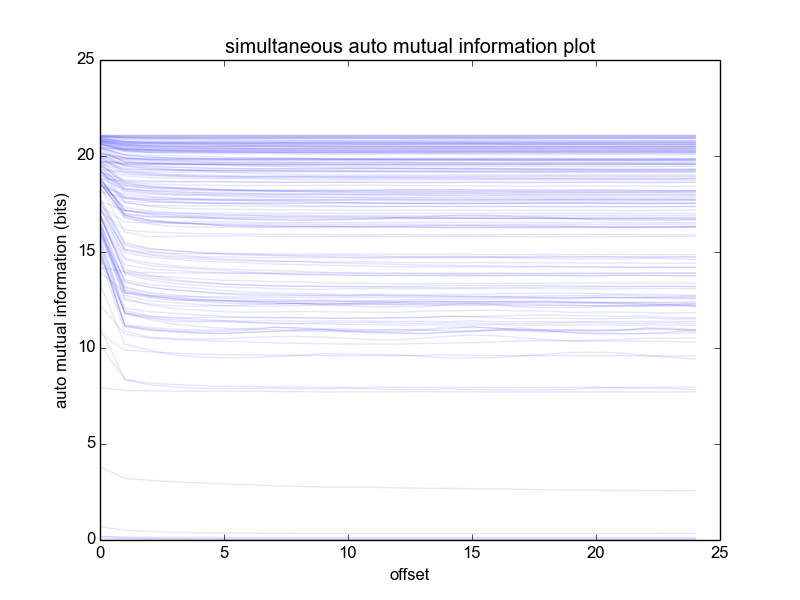
\includegraphics[scale=0.4]{wests_ami_mc}
    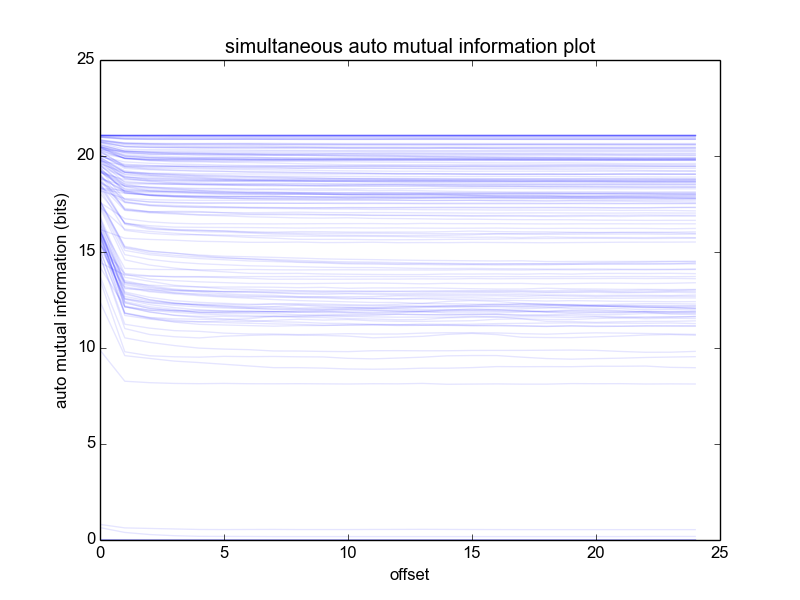
\includegraphics[scale=0.4]{norths_ami_mc}
    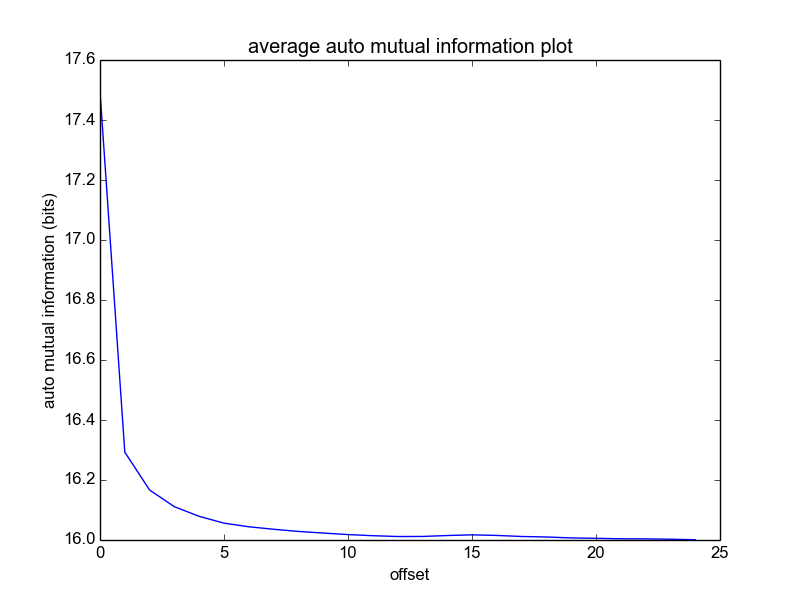
\includegraphics[scale=0.4]{wests_ami_summary}
    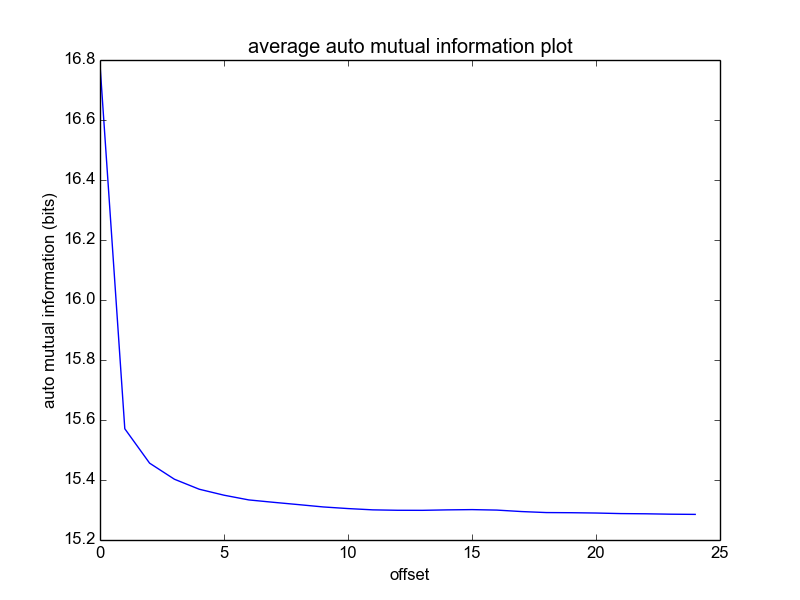
\includegraphics[scale=0.4]{norths_ami_summary}
  \end{center}
  \caption{Lagged amis: from left to right, west and north, west and north simultaneous and average plot}
\end{figure}

As can be seen, there exist clear patterns which stay constant over the lagging process of which time series are more close to each other with cross-mutual information, and clear differentiation between pairs.

\section{Frequency Domain}

There is more than one way to represent time series data, even given only the data itself and not any underlying function that generates it. We will show the use of the frequency representation in re-representing our data so that it shows a numerical current state of the phase, using the related Hilbert transform.

The frequency domain represents data in terms of the linear combination of simple sine and cosine waves: the analogy often used is that of a chord being hit on a piano, which can be represented with its time domain signal but can also be represented as the amplitude of the individual notes within the chord, which presents a better decomposition of the sound in and of itself. Likewise, we can attempt to decompose our time domain signals into the frequencies of the sinusoids which make it up.

The fast Fourier transform\cite{fft} is an essential tool for the further analyses below. It converts a finite discrete sample from the time to the frequency domain in a computable and fast way, and is generally an important workhorse algorithm in signals processing. An actual description of it is outside of the scope of this paper, but it works by dividing and conquering the discrete Fourier transform matrix into smaller ones, recursively, and recombining them.

\subsection{Hilbert Transform and $\gamma$}

A signal is called an \emph{analytic signal} if it does not have any negative-frequency components. The Hilbert transform is a way to get the analytic \emph{representation} for a signal in the time domain, which throws away the superfluous information which would be in a spectrum of that signal. This allows the expression of the analytic signal in terms of its time-variant magnitude and phase, allowing a study of the phase in an \emph{unwrapped form}\cite{gabor}. Why this is important is that it allows the measurement of phase synchronization, or synchronization of phase alone, apart from the more general phenomena of synchronization.

Formally speaking, given that the original signal is $s(t)$, the analytic signal $\zeta$ is:

$$\zeta(t) = s(t) + js_H(t) = A(t)e^{j\phi(t)}$$

$$s_H(t) = \frac{1}{\pi} PV \int_{-\infty}^{\infty} \frac{s(t)}{t - \tau} d\tau$$

$s_H$ is called the Hilbert transform; $PV$ indicates that the integral is a Cauchy principal value integral. The Hilbert transform is thus formally equivalent to convolution of $s(t)$ with $\frac{1}{\pi t}$, so in practice, it can easily be calculated from the fast Fourier transform, by taking the fast Fourier transform, taking the Fourier basis coefficients which correspond to negative frequencies with zeros, and taking the inverse Fourier transform of that result.\cite{hilbert}

\begin{figure}\label{fig:hilbert_plots}
  \begin{center}
    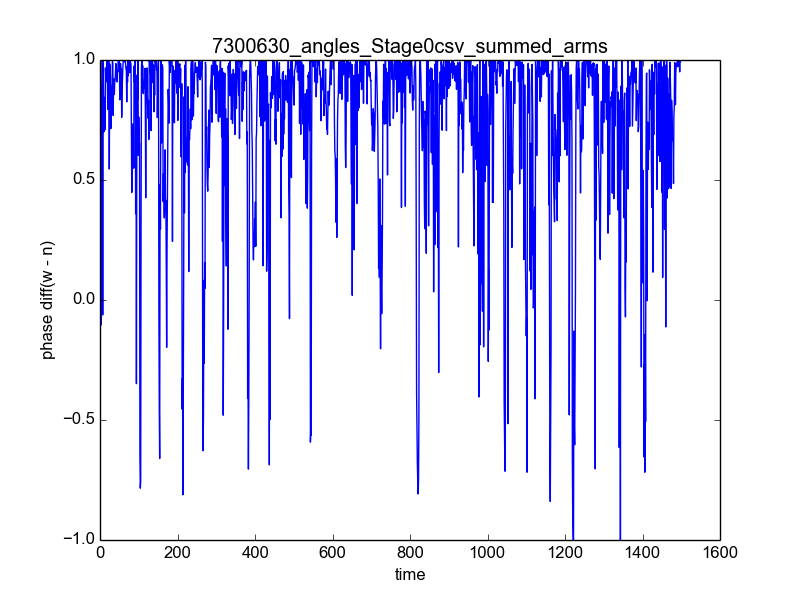
\includegraphics[scale=0.4]{hilbert_1}
    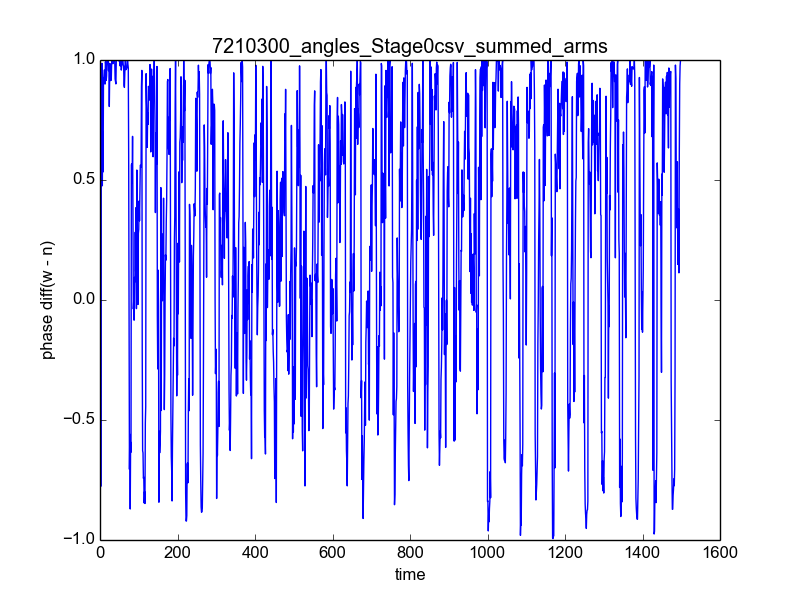
\includegraphics[scale=0.4]{hilbert_2}
    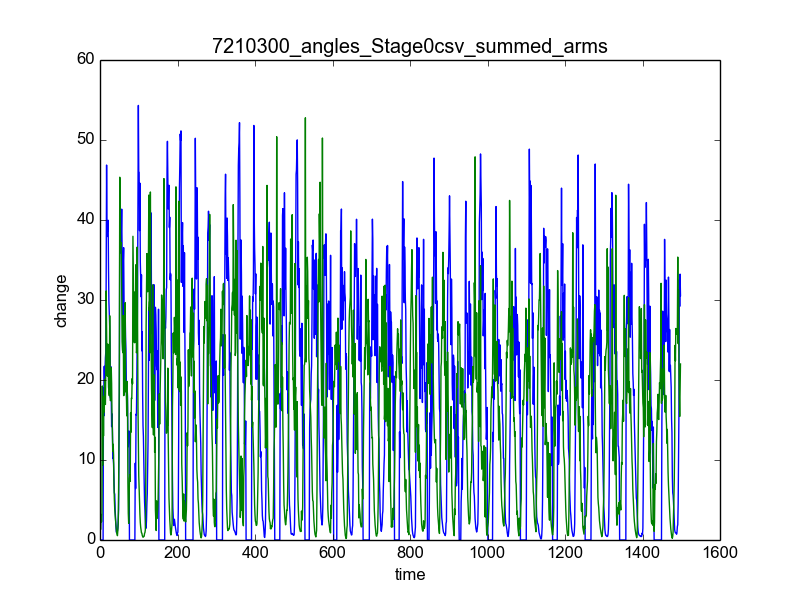
\includegraphics[scale=0.4]{time_1}
    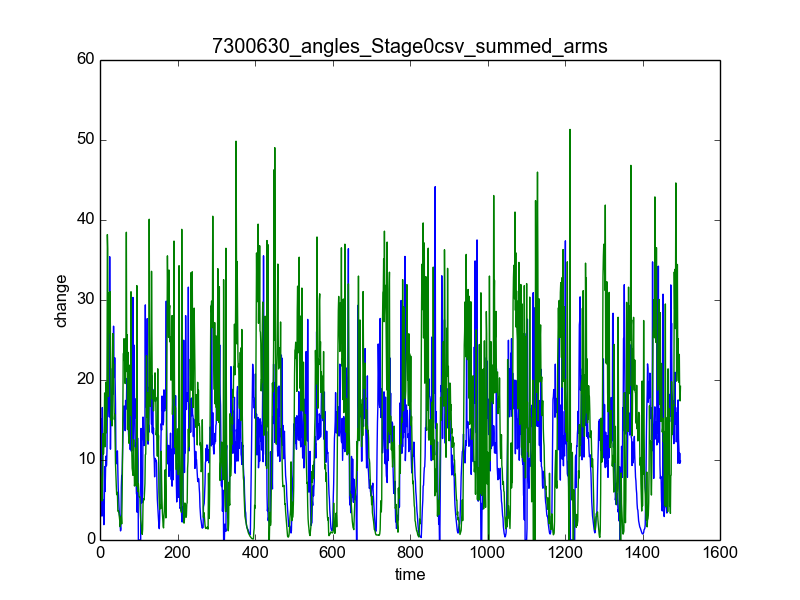
\includegraphics[scale=0.4]{time_2}
  \end{center}
  \caption{Example differences of Hilbert transforms from real data and the corresponding time domain data, note the periodicity}
\end{figure}

A derived statistic from the Hilbert transform for actually measuring synchronization between two instantaneous phases $\phi_x$ and $\phi_y$ is called $\gamma$ and is from \cite{gamma}. It is defined as:

$$ \gamma = |\langle e^{i(n\phi_x - m\phi_y)} \rangle| $$

\begin{figure}\label{fig:total_gammas}
  \begin{center}
    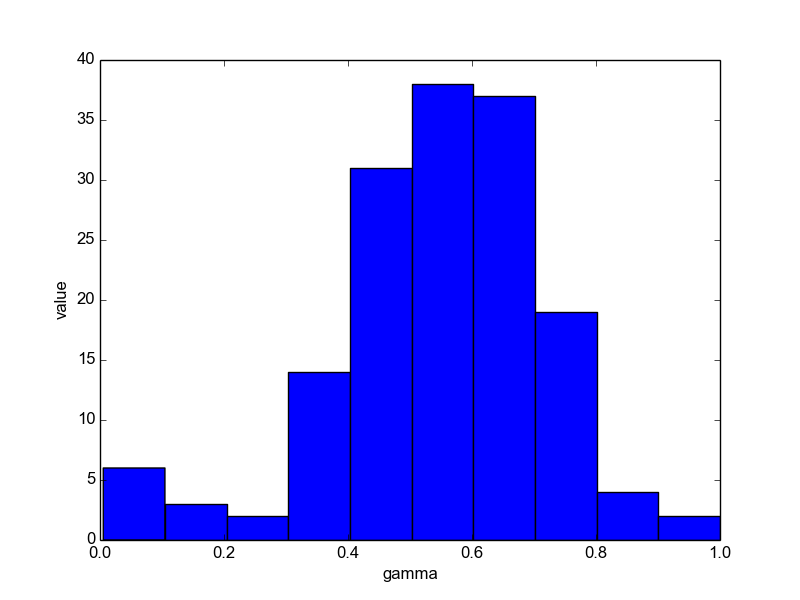
\includegraphics[scale=0.6]{total_gammas}
  \end{center}
  \caption{Histogram of gamma values in dataset}
\end{figure}

\section{Deterministic dual between discrete time series and ordered multigraph}

\subsection{Description}

There exists a line of analysis in the complex network literature which aims to convert a digital time series into a network. This is advantageous for analysis of time series because there is a deep and well-developed theory of networks: so far, an important result is that different time series result in networks with distinct topological properties, and that these topological properties relate to the time series in some way in addition to being determined by them\cite{campanharo}.

These methods are based upon a variety of features of the time series, such as correlational structure\cite{correlationgraph}, visibility\cite{lacasa}, phase space reconstruction\cite{phasespacegraph} and many others, which all attempt to differentiate time series by mapping them into networks with divergent properties. Notably, the degree distribution of the visibility graph is claimed in \cite{lacasa} to be related directly to the Fourier power spectrum of the time series, because the visibility graph depends upon the relation of peaks of the time series to one another.

Upon hearing of the mapping from a time series into a network, it might be wondered at if there exists a mapping from a network back into a time series. There does exist some methods to apply the inverse mapping, but none of these are deterministic, meaning that the network topology constrains the set of time series that the mapping can produce from that network, but does not completely determine it\cite{campanharo}. This is an undesirable property because the time series cannot be deterministically reproduced from the graph: what is reproduced is only a time series with statistical properties akin to that of the previous time series.

A deterministic transformation from time series to networks and from networks to time series can be made, however, if we allow duplication in the adjacencies of each vertex of the graph (making the graph a multigraph, by many definitions of multigraph\cite{multigraph}), and if we keep the order in which the vertices were travelled in the discrete time series. In addition to this, the start state of the time series must be stored.

In order to construct the labelled multigraph from a time series, the possible states of the time series, $\Sigma = {1 ... N}$ are made into the vertices of the multigraph. Then, starting with the value of the series at $t =1$, the vertices are traversed in the order that the corresponding states are traversed in the time series, and when one leaves a vertex $V_1$ to go to a vertex $V_2$, the identity of $V_2$ is pushed onto the list (like a stack) for the adjacencies of $V_1$ (\ref{fig:stackgraph}). There is pseudocode for this algorithm in \ref{fig:stackconstructionalgo}

In order to reconstruct the time series from a multigraph of this kind, therefore, we start from the start node again and consume the adjacency lists starting from the initial elements of the lists, to find the next node to jump to: this is detailed in \ref{fig:timeconstructionalgo}.

The model is very reminiscent of models from symbolic dynamics, just as \cite{campanharo} mentioned that their analysis was reminiscent of models from symbolic dynamics, because a continuous system is being discretized into a sequence of symbols representing the state of the system, which turn into nodes in a graph. Therefore, another important consideration is the size of the buckets which the time series is to be discretized into. For the examples below we chose bucket size of $0.05$ to discretize the time series, but this was not a principled decision and other methods, such as nearest neighbors, might be investigated, in an analogous way to the discretization of time series for determination of mutual information\cite{nnmi}.

\begin{figure}\label{fig:stackgraph}
  \begin{center}
    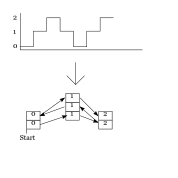
\includegraphics[scale=0.6]{stack_graph_ex}
  \end{center}
  \caption{Example construction of stack graph}
\end{figure}

\begin{figure}\label{fig:stackconstructionalgo}
  \begin{singlespace}
    \begin{verbatim}
    def time_series_to_stack_graph(data):
    stack_graph = graph in the form of list of lists
    for x, y in data bigrams:
        graph[x].append(y)
    return stack_graph, data[0] #must also have information about start
    \end{verbatim}
  \end{singlespace}
  \caption{Construction of stack graph from time series}
\end{figure}

\begin{figure}\label{fig:timeconstructionalgo}
\begin{singlespace}
\begin{verbatim}
def stack_graph_to_time_series(stack_graph, start):
    curr_idx = start
    path = [start]
    while length(stack_graph[curr_idx]) > 0:
        curr_member = stack_graph[curr_idx].pop_head()
        curr_idx = curr_member
        path.append(curr_member)
    return path
\end{verbatim}
\end{singlespace}
  \caption{Construction of time series from stack graph}
\end{figure}

\subsection{Implementation}

We will investigate the network properties of three toy models of a one-dimensional time series: a simple sinusoid, a chaotic logistic map, and a fractional Brownian motion. We will also investigate them on an exemplary time series from the dataset.

The concept of a node degree has a natural analog in the stack graph, where the outdegree number for each node is the size of the corresponding stack (as opposed to the cardinality of the set of outgoing edges, which is a set and doesn't have duplicates). However, the clustering coefficient and average shortest path length of the stack graph do not have as immediately obvious meanings and therefore we took those statistics on a graph induced on the stack graph, where each stack had duplicates removed and therefore turned into a set of tails on the outdegree. This ends up being something like the recurrence matrix construction\cite{recurrencegraph} of a network from the time series, and is an information-losing operation.

\begin{figure}\label{fig:stack_ts_plots}
  \begin{center}
    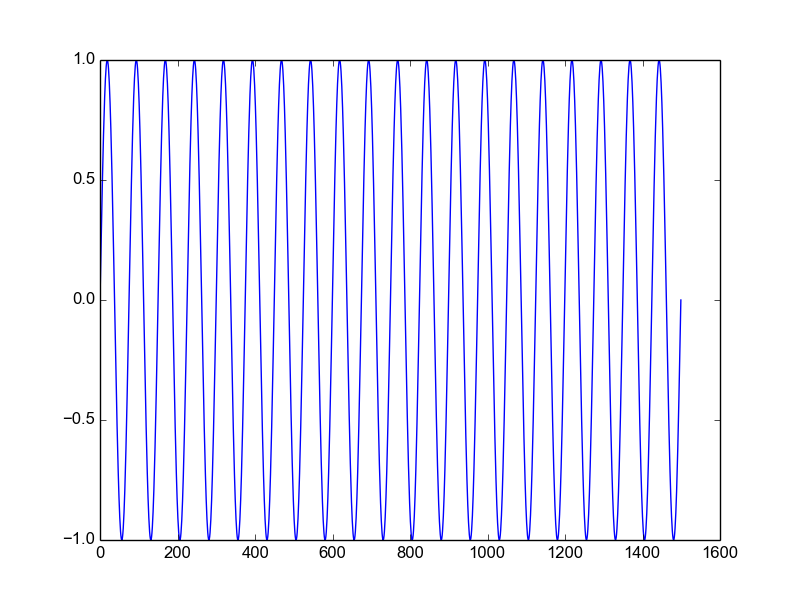
\includegraphics[scale=0.4]{plot_sinusoid}
    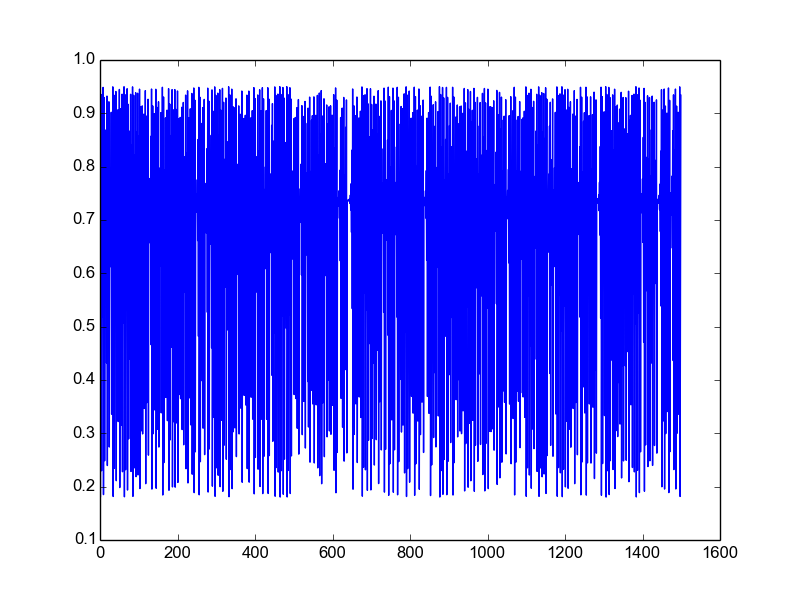
\includegraphics[scale=0.4]{plot_logistic}
    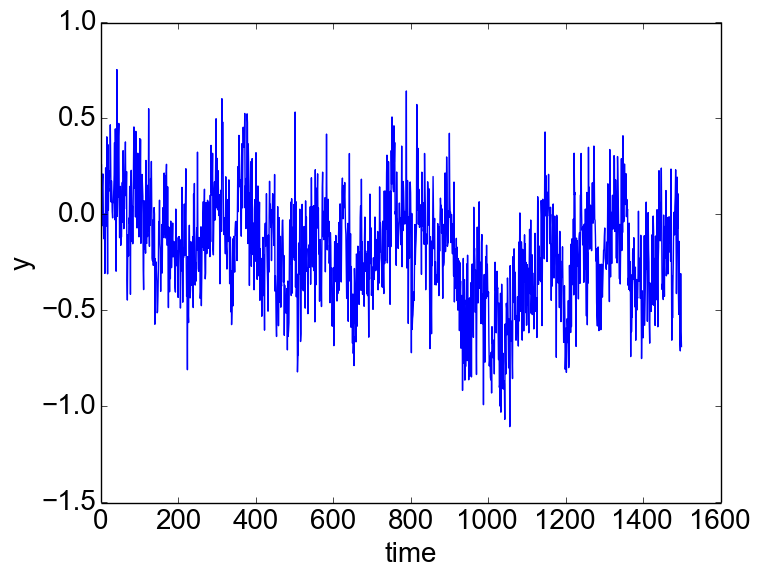
\includegraphics[scale=0.4]{plot_fbm}
    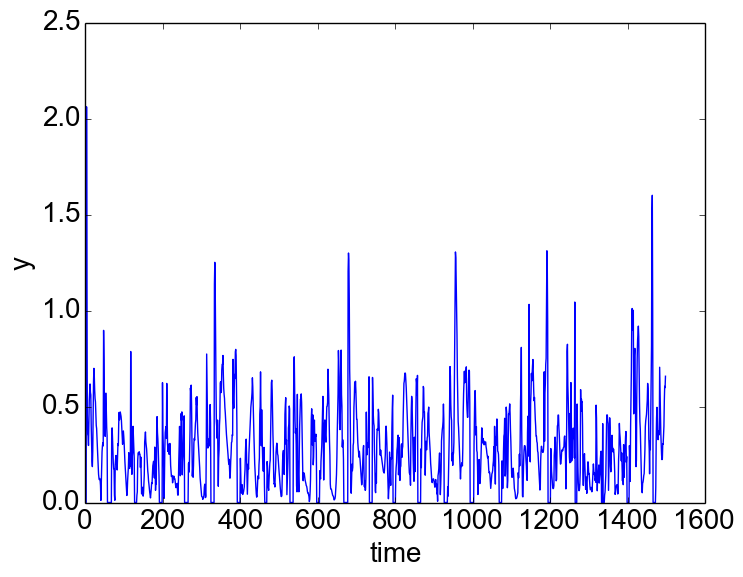
\includegraphics[scale=0.4]{plot_vr}
  \end{center}
  \caption{Plotted series in time domain. From left to right: sinusoid, logistic map with full chaos (r=3.8), fractional Brownian motion, real data}
\end{figure}
\begin{figure}\label{fig:stack_ts_spectra}
  \begin{center}
    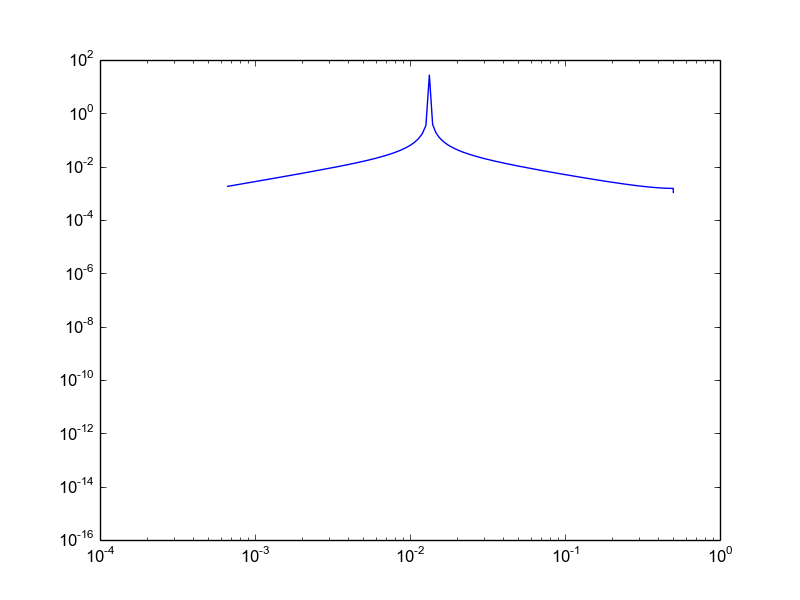
\includegraphics[scale=0.4]{spectrum_sinusoid}
    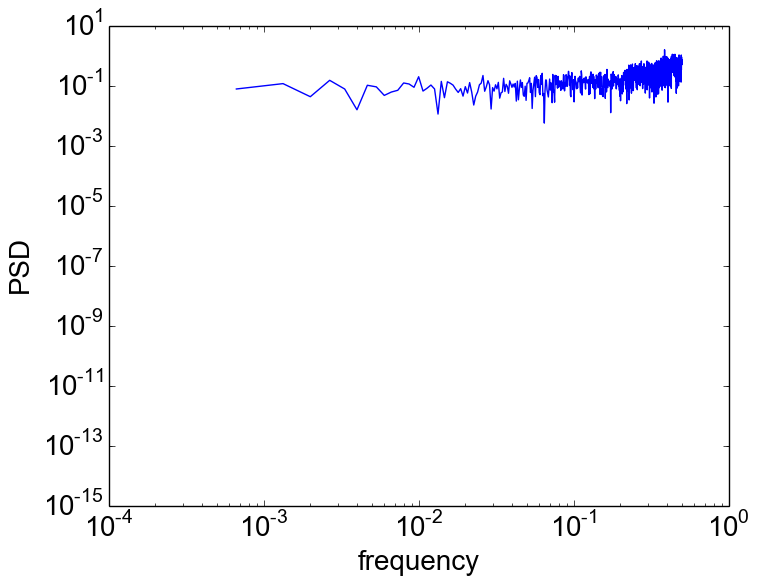
\includegraphics[scale=0.4]{spectrum_logistic}
    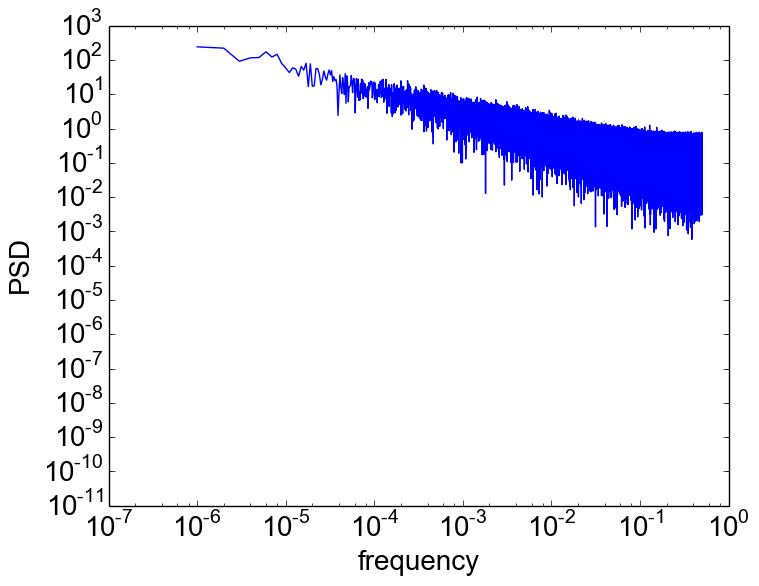
\includegraphics[scale=0.4]{spectrum_fbm}
    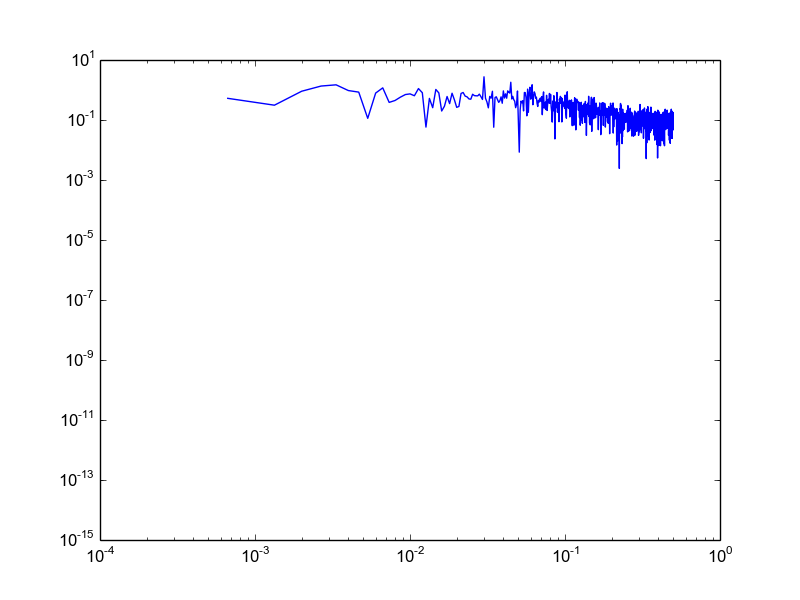
\includegraphics[scale=0.4]{spectrum_vr}
  \end{center}
  \caption{Plotted series in frequency domain. From upper left to lower right: sinusoid, logistic map with full chaos (r=3.8), fractional Brownian motion, real data}
\end{figure}
\begin{figure}\label{fig:stack_ts_degree}
  \begin{center}
    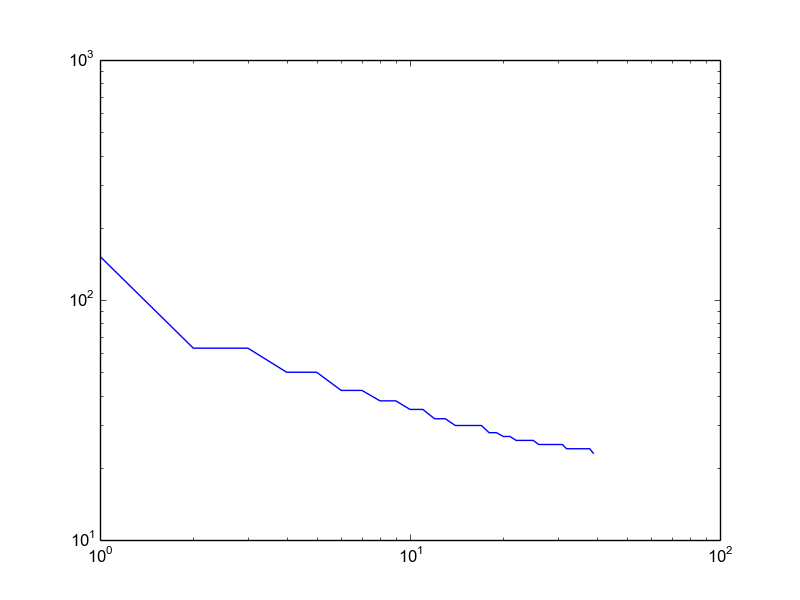
\includegraphics[scale=0.4]{degrees_sinusoid}
    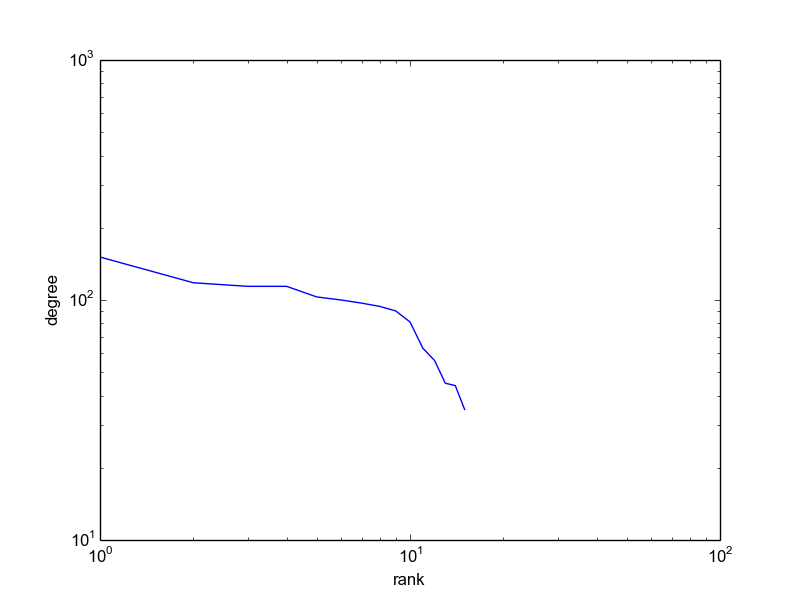
\includegraphics[scale=0.4]{degrees_logit}
    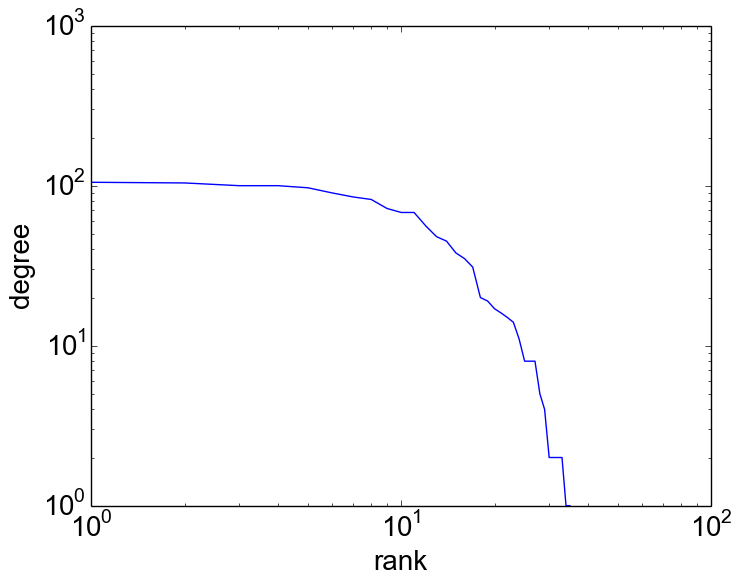
\includegraphics[scale=0.4]{degrees_fbm}
    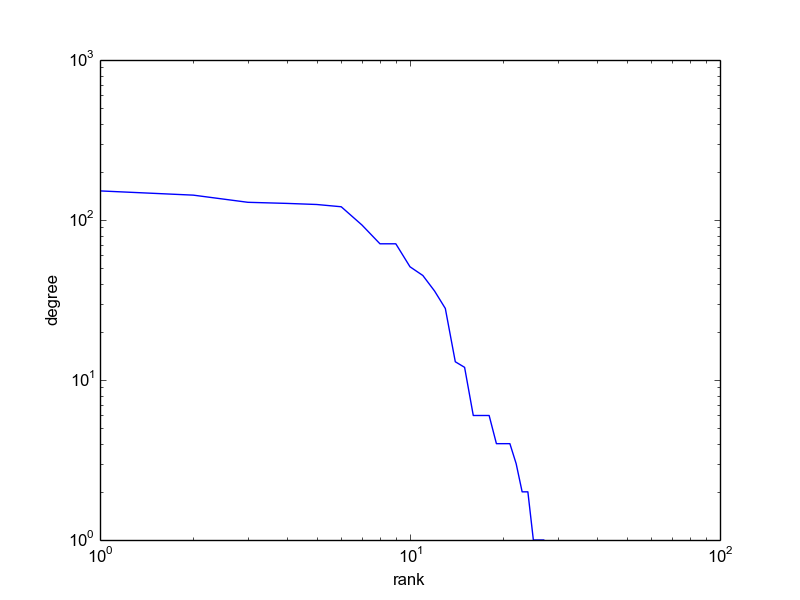
\includegraphics[scale=0.4]{degrees_vr}
  \end{center}
  \caption{Equivalent degree distribution in stack graph. From upper left to lower right: sinusoid, logistic map with full chaos (r=3.8), fractional Brownian motion, real data}
\end{figure}
\begin{figure}\label{fig:resampled_stack}
  \begin{center}
    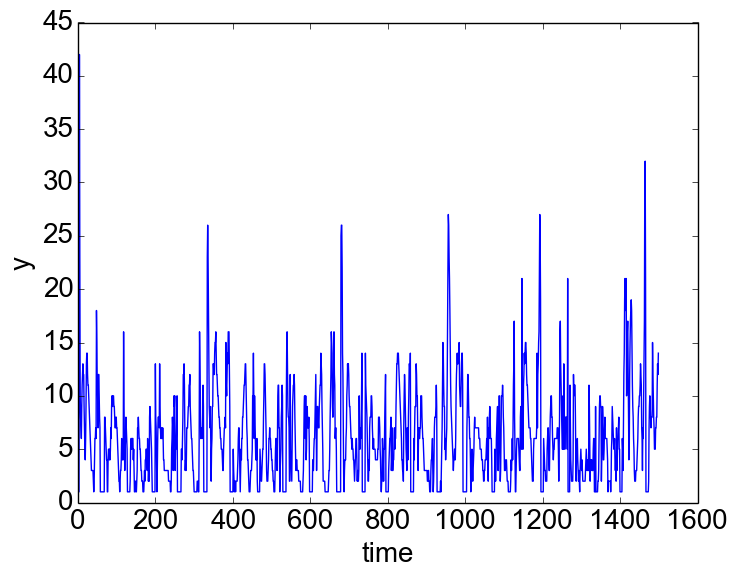
\includegraphics[scale=0.6]{resampled_stack}
  \end{center}
  \caption{Time series transformed back from the stack graph. Note discretization.}
\end{figure}

\begin{figure}\label{fig:stack_ts_others}
  \begin{tabular} {c || c c c c}
    Measure & Sinusoid & Logistic Map & FBM & Real Data \\
    Clustering Coefficient & 0.425 & 0.092 & 0.768 & 0.572 \\
    Average Shortest Path Length & 7.38 & 2.67 & 1.85 & 2.27 \\
  \end{tabular}
  \caption{Other properties of stack graph, after flattening}
\end{figure}

\subsection{Acknowledgements}

Thanks to Jeremy Bailenson for advising, and to Andrea Stevenson Won for the data used in this analysis, and to the Virtual Human Interaction Lab more generally. Also, thanks to my friends and family.

\begin{thebibliography}{}
  \bibitem{syncreview}
    Repp, B. H. (2005). Sensorimotor synchronization: a review of the tapping literature. Psychonomic bulletin \& review, 12(6), 969-992.
  \bibitem{physsync}
    Pikovsky, A., Rosenblum, M., \& Kurths, J. (2001). A universal concept in nonlinear sciences. Self, 2, 3.
  \bibitem{socialsync}
    Delaherche, E., Chetouani, M., Mahdhaoui, A., Saint-Georges, C., Viaux, S., \& Cohen, D. (2012). Interpersonal synchrony: A survey of evaluation methods across disciplines. Affective Computing, IEEE Transactions on, 3(3), 349-365.
  \bibitem{andrea}
    Won, A. S., Bailenson, J. N., Stathatos, S. C., \& Dai, W. (2014). Automatically detected nonverbal behavior predicts creativity in collaborating dyads. Journal of Nonverbal Behavior, 38(3), 389-408.
  \bibitem{coop}
    Wiltermuth, S. S., \& Heath, C. (2009). Synchrony and cooperation. Psychological science, 20(1), 1-5.
  \bibitem{rapport}
    Gratch, J., Wang, N., Gerten, J., Fast, E., \& Duffy, R. (2007, January). Creating rapport with virtual agents. In Intelligent Virtual Agents (pp. 125-138). Springer Berlin Heidelberg.
  \bibitem{goals}
    Semin, G. R., \& Cacioppo, J. T. (2008). Grounding social cognition: Synchronization, entrainment, and coordination. Embodied grounding: Social, cognitive, affective, and neuroscientific approaches, 119-147.
  \bibitem{campanharo}
    Campanharo, A. S., Sirer, M. I., Malmgren, R. D., Ramos, F. M., \& Amaral, L. A. N. (2011). Duality between time series and networks. PloS one, 6(8), e23378.
  \bibitem{multigraph}
    West, D. B. (2001). Introduction to graph theory (Vol. 2). Upper Saddle River: Prentice hall.
  \bibitem{manual}
    Feldman, R. (1998). Coding interactive behavior manual. Unpublished manual.
  \bibitem{manualval}
    Feldman, R. (2007). Parent–infant synchrony and the construction of shared timing; physiological precursors, developmental outcomes, and risk conditions. Journal of Child psychology and Psychiatry, 48(3‐4), 329-354.
  \bibitem{blascovich}
    Loomis, J. M., Blascovich, J. J., \& Beall, A. C. (1999). Immersive virtual environment technology as a basic research tool in psychology. Behavior Research Methods, Instruments, \& Computers, 31(4), 557-564.
  \bibitem{pompe}
    Pompe, B., Blidh, P., Hoyer, D., \& Eiselt, M. (1998). Using mutual information to measure coupling in the cardiorespiratory system. Engineering in Medicine and Biology Magazine, IEEE, 17(6), 32-39.
  \bibitem{hrv1}
    Kamen, P. W., \& Tonkin, A. M. (1995). Application of the Poincare plot to heart rate variability: a new measure of functional status in heart failure. Australian and New Zealand journal of medicine, 25(1), 18-26.
  \bibitem{pushdown}
    Autebert, J. M., Berstel, J., \& Boasson, L. (1997). Context-free languages and pushdown automata. In Handbook of formal languages (pp. 111-174). Springer Berlin Heidelberg.
  \bibitem{gabor}
    Gabor, D. (1946). Theory of communication. Part 1: The analysis of information. Journal of the Institution of Electrical Engineers-Part III: Radio and Communication Engineering, 93(26), 429-441.
  \bibitem{pressing}
    Pressing, J. (1999). The referential dynamics of cognition and action. Psychological Review, 106(4), 714.
  \bibitem{schulze}
    Vorberg, D., \& Schulze, H. H. (2002). Linear phase-correction in synchronization: Predictions, parameter estimation, and simulations. Journal of Mathematical Psychology, 46(1), 56-87.
  \bibitem{bellman}
    Bellman, R. (1956). Dynamic programming and Lagrange multipliers. Proceedings of the National Academy of Sciences of the United States of America, 42(10), 767.
  \bibitem{mates}
    Mates, J. (1994). A model of synchronization of motor acts to a stimulus sequence. Biological cybernetics, 70(5), 463-473.
  \bibitem{hary}
    Hary, D., \& Moore, G. P. (1987). Synchronizing human movement with an external clock source. Biological cybernetics, 56(5-6), 305-311.
  \bibitem{correlationgraph}
    Zhang, J., \& Small, M. (2006). Complex network from pseudoperiodic time series: Topology versus dynamics. Physical Review Letters, 96(23), 238701.
  \bibitem{lacasa}
    Lacasa, L., Luque, B., Ballesteros, F., Luque, J., \& Nuño, J. C. (2008). From time series to complex networks: The visibility graph. Proceedings of the National Academy of Sciences, 105(13), 4972-4975.
  \bibitem{phasespacegraph}
    Gao, Z., \& Jin, N. (2009). Complex network from time series based on phase space reconstruction. Chaos: An Interdisciplinary Journal of Nonlinear Science, 19(3), 033137.
  \bibitem{nnmi}
    Kraskov, A., Stögbauer, H., \& Grassberger, P. (2004). Estimating mutual information. Physical review E, 69(6), 066138.
  \bibitem{alzheimersmi}
    Jeong, J., Gore, J. C., \& Peterson, B. S. (2001). Mutual information analysis of the EEG in patients with Alzheimer's disease. Clinical Neurophysiology, 112(5), 827-835.
  \bibitem{anscombe}
    Anscombe, F. J. (1973). Graphs in statistical analysis. The American Statistician, 27(1), 17-21.
  \bibitem{recurrencegraph}
    Donner, R. V., Zou, Y., Donges, J. F., Marwan, N., \& Kurths, J. (2010). Recurrence networks—a novel paradigm for nonlinear time series analysis. New Journal of Physics, 12(3), 033025.
  \bibitem{framedifferencing}
    Paxton, A., \& Dale, R. (2013). Frame-differencing methods for measuring bodily synchrony in conversation. Behavior research methods, 45(2), 329-343.
  \bibitem{webber}
    Webber, C. L., \& Zbilut, J. P. (1994). Dynamical assessment of physiological systems and states using recurrence plot strategies. Journal of applied physiology, 76(2), 965-973.
  \bibitem{musicians}
    Camurri, A., Varni, G., \& Volpe, G. (2009, September). Measuring entrainment in small groups of musicians. In Affective Computing and Intelligent Interaction and Workshops, 2009. ACII 2009. 3rd International Conference on (pp. 1-4). IEEE.
  \bibitem{puzzles}
    Shockley, K., Santana, M. V., \& Fowler, C. A. (2003). Mutual interpersonal postural constraints are involved in cooperative conversation. Journal of Experimental Psychology: Human Perception and Performance, 29(2), 326.
  \bibitem{richardson}
    Richardson, M. J., Marsh, K. L., Isenhower, R. W., Goodman, J. R., \& Schmidt, R. C. (2007). Rocking together: Dynamics of intentional and unintentional interpersonal coordination. Human movement science, 26(6), 867-891.
  \bibitem{movementfeatures}
    Delaherche, E., \& Chetouani, M. (2010, October). Multimodal coordination: exploring relevant features and measures. In Proceedings of the 2nd international workshop on Social signal processing (pp. 47-52). ACM.
  \bibitem{movementparts}
    Oullier, O., De Guzman, G. C., Jantzen, K. J., Lagarde, J., \& Scott Kelso, J. A. (2008). Social coordination dynamics: Measuring human bonding. Social neuroscience, 3(2), 178-192.
  \bibitem{imageprocessing}
    Ashenfelter, K. T., Boker, S. M., Waddell, J. R., \& Vitanov, N. (2009). Spatiotemporal symmetry and multifractal structure of head movements during dyadic conversation. Journal of Experimental Psychology: Human Perception and Performance, 35(4), 1072.
  \bibitem{videotracking}
    Campbell, N. (2008, December). Multimodal Processing of Discourse Information; The Effect of Synchrony. In ISUC (pp. 12-15).
  \bibitem{gamma}
    Lachaux, J. P., Rodriguez, E., Martinerie, J., \& Varela, F. J. (1999). Measuring phase synchrony in brain signals. Human brain mapping, 8(4), 194-208.
  \bibitem{hilbert}
    Hahn, S. L. (1996). Hilbert transforms in signal processing. Artech House on Demand.
  \bibitem{kamen}
    Brennan, M., Palaniswami, M., \& Kamen, P. (2001). Do existing measures of Poincare plot geometry reflect nonlinear features of heart rate variability?. Biomedical Engineering, IEEE Transactions on, 48(11), 1342-1347.
  \bibitem{fft}
    Cooley, J. W., \& Tukey, J. W. (1965). An algorithm for the machine calculation of complex Fourier series. Mathematics of computation, 19(90), 297-301.
\end{thebibliography}

\end{document}
